\documentclass[a4paper,10pt]{article}

\usepackage[top=0.75in, bottom=0.75in, left=0.55in, right=0.85in]{geometry}
\usepackage{graphicx}
\usepackage{url}
\usepackage{palatino}
\usepackage{tabularx}

\fontfamily{SansSerif}
\selectfont

\usepackage[T1]{fontenc}
\usepackage
[utf8]
{inputenc}

\usepackage{color}
\definecolor{mygrey}{gray}{0.75}
\textheight=9.75in
\raggedbottom

\setlength{\tabcolsep}{0in}
\newcommand{\isep}{-2 pt}
\newcommand{\lsep}{-0.5cm}
\newcommand{\psep}{-0.6cm}
\renewcommand{\labelitemii}{$\circ$}

\pagestyle{empty}

\newcommand{\resitem}[1]{\item #1 \vspace{-2pt}}
\newcommand{\resheading}[1]{{\small \colorbox{mygrey}{\begin{minipage}{0.975\textwidth}{\textbf{#1 \vphantom{p\^{E}}}}\end{minipage}}}}
\newcommand{\ressubheading}[3]{
\begin{tabular*}{6.62in}{l @{\extracolsep{\fill}} r}
	\textsc{{\textbf{#1}}} & \textsc{\textit{[#2]}} \\
\end{tabular*}\vspace{-8pt}}


\begin{document}
\hspace{0.5cm}\\[-0.2cm]
\indent \Large \textbf{Gopala Dhar} \\         
\normalsize
\indent 27/37 Manish Nagar, \\
\indent Four Bungalows, Andheri W,  \\                                                                                                                                                                                                                                                           
\indent Mumbai (Maharashtra, INDIA) - 400053\\
\indent Email-Id : \textbf{dhargopala@gmail.com} \\
\indent Mobile No.: \textbf{9930350113} \\
\indent Alt Mob No.: \textbf{9419192948} \hfill
\smash{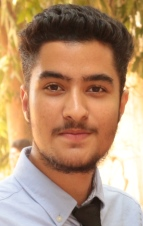
\includegraphics[scale=0.5]{Gopala.jpg}}\\  


\resheading{\textbf{CAREER OBJECTIVE} }\\[\lsep]\\\\
\indent As an \textit{Electronics Engineer}, in my Second Year, I've developed a urge for practical knowledge, be it working \indent on algorithms or interfacing Sensors.\par I Believe that \textbf{Automation} is the future and would like to pursue a Career in Automation with implementation \par of \textit{Machine Learning} and \textit{Neural Networks} along with \textit{Computer Vision}. \par I foresee its Implementation to solve Real Word issues and I would be gratified if I could help the World \par become a better Place.\\

\resheading{\textbf{ACADEMIC DETAILS} }\\[\lsep]
\\ \\
\indent \begin{tabular}{ l @{\hskip 0.15in} l @{\hskip 0.15in} l @{\hskip 0.15in} l @{\hskip 0.15in} l }
\hline\\
\textbf{Examination} & \textbf{University/Board} & \textbf{Institute} & \textbf{Year} & \textbf{CGPA/\%} \\
\hline\\
Undergraduate& \textit{Autonomous}&Sardar Patel Institute of Technology, Mumbai&2018&Pursuing \\
(4th Sem, Electronics)&\textit{(Mumbai University)}&&& \\
Undergraduate& \textit{Autonomous}&Sardar Patel Institute of Technology, Mumbai&2017&10 \\
(3rd Sem, Electronics)&\textit{(Mumbai University)}&&& \\
Undergraduate& \textit{Mumbai University}&Sardar Patel Institute of Technology, Mumbai&2017&9.04 \\
(1st Year, Electronics)&&&& \\
Higher Secondary& \textit{CBSE}& Delhi Public School, Jammu&2016&91.2 \\
Matriculation & \textit{CBSE}& Delhi Public School, Jammu&2014&10 \\

\hline
\end{tabular}
\\\\
\indent \resheading{\textbf{PROJECTS AND COMPETITIONS} }\\\\[\lsep]
\begin{enumerate}

\item eYRC (2017)
\item Robocon (2016, 2017)
\item Land Mine Detection and Mapping (IICDC 2017)
\end{enumerate}

\resheading{\textbf{TRAINING AND INTERNSHIP} }\\\\[\lsep]
\begin{itemize}
\item College Certified Course in \textbf{LabVIEW}
\item College Certified Course in \textbf {Verilog}
\end{itemize}

\resheading{\textbf{RESEARCH PUBLICATIONS} }\\\\[\lsep]
\begin{enumerate}
\item BDR problem solving through SIMULINK and MATLAB has been taken up and outcome of results will be submitted for publication during this year
\end{enumerate}

\resheading{\textbf{TECHNICAL SKILLS} }\\\\[\lsep]
\begin{itemize}
\item Possess hands on experience of Micro-controllers and Micro Computers such as Arduino, Raspberry Pi etc
\item Indepth working knowledge of Image Processing through Open-CV
\item Interfacing experience of a Host of Sensors including IR Arrays, Lidar Sensor, Ultrasonic Module etc
\item Well versed with Pneumatics and  DC motors including BLDC, Steppers and Servos
\item Ability to design basic Circuits and Drivers
\item Familiar with Languages: C, Python, VHDL, Verilog
\end{itemize}

\resheading{\textbf{SOFT SKILLS} }\\\\[\lsep]
\begin{enumerate}
\item Very good ability to work in a Team
\item Possess excellent Communication Skills
\item Problem Solving and Time Management attitude
\end{enumerate}

\resheading{\textbf{EXTRA- CURRICULAR ACTIVITIES} }\\\\[\lsep]
\begin{itemize}
\item Member of Fire and Security Association of India
\item Active Participent of Versova Beach Clean Drive
\item Avid Badminton Player
\end{itemize}

\resheading{\textbf{CO- CURRICULAR ACTIVITIES} }\\\\[\lsep]
\begin{enumerate}
\item Member of the College Robocon Team From The Past Two Years
\item Organized Technical workshop for Juniors
\end{enumerate}

\resheading{\textbf{PERSONAL DETAILS} }\\\\[\lsep]

\indent Father's Name:   Dr. Anil Dhar\\ 
\indent Mother's Name:   Dr. Asha Dhar\\
\indent Sex:   Male\\
\indent Date of Birth:   29th October,1998\\
\indent Nationality:   Indian\\
\indent Marital Status:   Unmarried\\

\resheading{\textbf{REFERENCE} }\\\\[\lsep]

\indent Dr. S.S. Rathod, \\
\indent Ph.D. (IIT, Roorkee), \\
\indent Dean Academics, \\
\indent Sardar Patel Institue of Technology, Mumbai\\
\indent Email: surendra\textunderscore rathod@spit.ac.in\\
\indent Mobile: 9920228275



\end{document}